%% ===================== 4. THIẾT LẬP =====================
\section{Thiết lập thực nghiệm}\label{sec:setup}

Thí nghiệm gồm hai bước, theo loại hình Applied Experimentation (Mục~\ref{sec:method}). Bước thứ nhất tái lập một bộ phát hiện kiểu DeSFAM (VAE + Isolation Forest, huấn luyện normal-only) trên dữ liệu thực DongTing và đánh giá năng lực phát hiện (RQ1). Bước thứ hai, trên chính dòng anomaly score của bộ phát hiện ấy, dựng một thí nghiệm đối kháng có kiểm soát: thao tác cường độ nhiễu của noisy neighbor và đối chứng ba chính sách ngưỡng trên \textit{cùng} một dòng dữ liệu (RQ2). Toàn bộ được thực hiện trên một pipeline ba phase tách biệt (train / calibrate / test rời rạc) nhằm loại rò rỉ dữ liệu. Các tiểu mục dưới đây trình bày lần lượt: dữ liệu, bộ phát hiện và trích xuất đặc trưng, mô hình mối đe doạ và hàng xóm gây nhiễu, và cuối cùng là quy trình ba phase cùng giao thức thí nghiệm.

\subsection{Dữ liệu}
Báo cáo sử dụng tập DongTing~\cite{dongting2023} ở dạng đã mã hoá (chuỗi system call ID theo bảng kernel 5.17): 5.105 chuỗi lành tính cho training, 656 chuỗi lành tính cho calibration và đánh giá, 6.436 chuỗi tấn công cho đánh giá. Đây là dữ liệu system call \textit{thực}, không phải dữ liệu tổng hợp.

\subsection{Bộ phát hiện và trích xuất đặc trưng}
\subsubsection{Bộ lọc sensor-alphabet: cơ chế, lý do và độ phủ}
Báo cáo áp dụng \textit{sensor-alphabet filter} (bảng chữ cái cảm biến) — chỉ giữ lại 24 system call liên quan an ninh (\texttt{execve, clone, setuid/setgid/capset, openat, unlinkat, renameat2, mount, unshare, setns, pivot\_root, socket, connect, bind, mprotect, mmap, prctl, memfd\_create, splice, ptrace, init/finit\_module, bpf}) — \textit{trước khi} windowing (độ dài 10, bước 2). Nhóm này chỉ chiếm $\sim 20\%$ system call ở chuỗi lành tính và $\sim 10\%$ ở chuỗi tấn công, song lại \textit{tập trung} tín hiệu privilege escalation.

Việc lọc trước khi windowing là cần thiết vì nhiều lý do hội tụ. Trước hết, nó \textit{tập trung tín hiệu và chống dilution}: dấu hiệu privilege escalation tập trung ở một nhóm nhỏ system call đặc quyền, trong khi workload lành tính bị áp đảo bởi \texttt{read/write/close/futex}; nếu đưa toàn bộ không gian system call vào, các call đặc quyền hiếm bị pha loãng đến mức mô hình normal-only không còn phân tách được benign với attack — thực nghiệm xác nhận điều này khi AUC tăng từ $0{,}504$ (không filter, gần như ngẫu nhiên) lên $0{,}832$ (có filter). Thứ hai, nó \textit{đồng bộ giữa huấn luyện và vận hành}: TracingPolicy của Tetragon khi triển khai chỉ trace đúng nhóm system call an ninh này, nên feature space lúc huấn luyện (trên DongTing) trùng khớp với tín hiệu cảm biến lúc vận hành. Thứ ba, nó \textit{giảm chi phí xử lý}: \texttt{read/write/futex} là các system call có tần suất cao nhất, loại bỏ chúng giúp giảm mạnh khối lượng tính toán, phù hợp với mục tiêu overhead $<1\%$ của DeSFAM. Cuối cùng, việc dùng binary presence trên một tập đặc quyền được tuyển chọn khiến kẻ tấn công khó \textit{pha loãng} tín hiệu bằng cách bơm thêm system call lành tính.

Tập 24 system call này được tuyển chọn để bao trọn các system call \textit{điều phối ranh giới đặc quyền}:
\begin{itemize}[leftmargin=1.2cm,itemsep=1pt]
\item đổi định danh / capability: \texttt{setuid, setgid, capset, prctl};
\item thao tác namespace--mount (container escape): \texttt{unshare, setns, pivot\_root, mount};
\item injection / tracing tiến trình: \texttt{ptrace}; nạp mã kernel: \texttt{init\_module, finit\_module, bpf};
\item execution: \texttt{execve, clone}; truy cập tệp nhạy cảm: \texttt{openat, unlinkat, renameat2};
\item memory permission: \texttt{mprotect, mmap, memfd\_create}; di chuyển dữ liệu: \texttt{splice}; network: \texttt{socket, connect, bind}.
\end{itemize}
Mọi kỹ thuật privilege escalation (TA0004) và container escape đều phải đi qua ít nhất một trong các ``kernel choke point'' này, nên 24 system call là \textit{đủ phủ} cho lớp tấn công được nghiên cứu. Bằng chứng định lượng: detector đạt AUC $0{,}832$, xấp xỉ mức DeSFAM-test ($\approx 0{,}835$), chỉ với feature space dựa trên 24 system call này. \textit{Giới hạn (xem Mục~\ref{sec:discuss}):} đây là một tập được tuyển chọn theo định hướng an ninh (khớp với TracingPolicy của Tetragon khi triển khai) chứ không nhằm liệt kê đầy đủ; một tấn công hoạt động hoàn toàn qua các system call ngoài tập (ví dụ \texttt{io\_uring} hoặc kênh data-only) sẽ không được quan sát — vì vậy mở rộng sensor alphabet là một hướng phát triển.

\subsubsection{Trích xuất đặc trưng}
Mỗi cửa sổ trượt (độ dài tối đa 10, chỉ gồm system call thuộc sensor alphabet 24 phần tử) được biểu diễn thành một feature vector 42 chiều, ghép từ ba khối (minh hoạ ở Hình~\ref{fig:fe}):
\begin{itemize}[leftmargin=1.2cm,itemsep=2pt]
\item \textbf{Tần suất (24 chiều):} tỷ lệ xuất hiện của mỗi system call trong alphabet, tính bằng số lần xuất hiện chia cho độ dài cửa sổ.
\item \textbf{Binary presence (15 chiều):} với 15 system call đặc quyền \textit{hiếm} (setuid/setgid/capset, unshare, setns, pivot\_root, mount, ptrace, init/finit\_module, bpf, memfd\_create, splice, renameat2, unlinkat), mỗi chiều chỉ ghi nhận \textit{có hay không} xuất hiện ($1$/$0$), thay vì đếm tần suất. Cách này nhằm \textbf{chống dilution}: một \texttt{ptrace} đơn lẻ trong một cửa sổ đầy \texttt{openat} vẫn ``lật bit'', trong khi tần suất sẽ làm chìm tín hiệu hiếm này.
\item \textbf{Thống kê (3 chiều):} entropy của phân phối tần suất, tỷ lệ số system call khác nhau trên 24, và tần suất lớn nhất — phản ánh mức độ đa dạng và tập trung của cửa sổ.
\end{itemize}
Toàn bộ vector được chuẩn hoá bằng RobustScaler (theo khoảng phân vị $p1$–$p99$), \textit{fit chỉ trên} cửa sổ normal-train. Quá trình huấn luyện và vận hành dùng \textit{cùng} một feature space 42 chiều — điều kiện để mô hình học trên DongTing áp dụng được cho dòng cửa sổ ở phase test/triển khai.

\begin{figure}[ht]
\centering
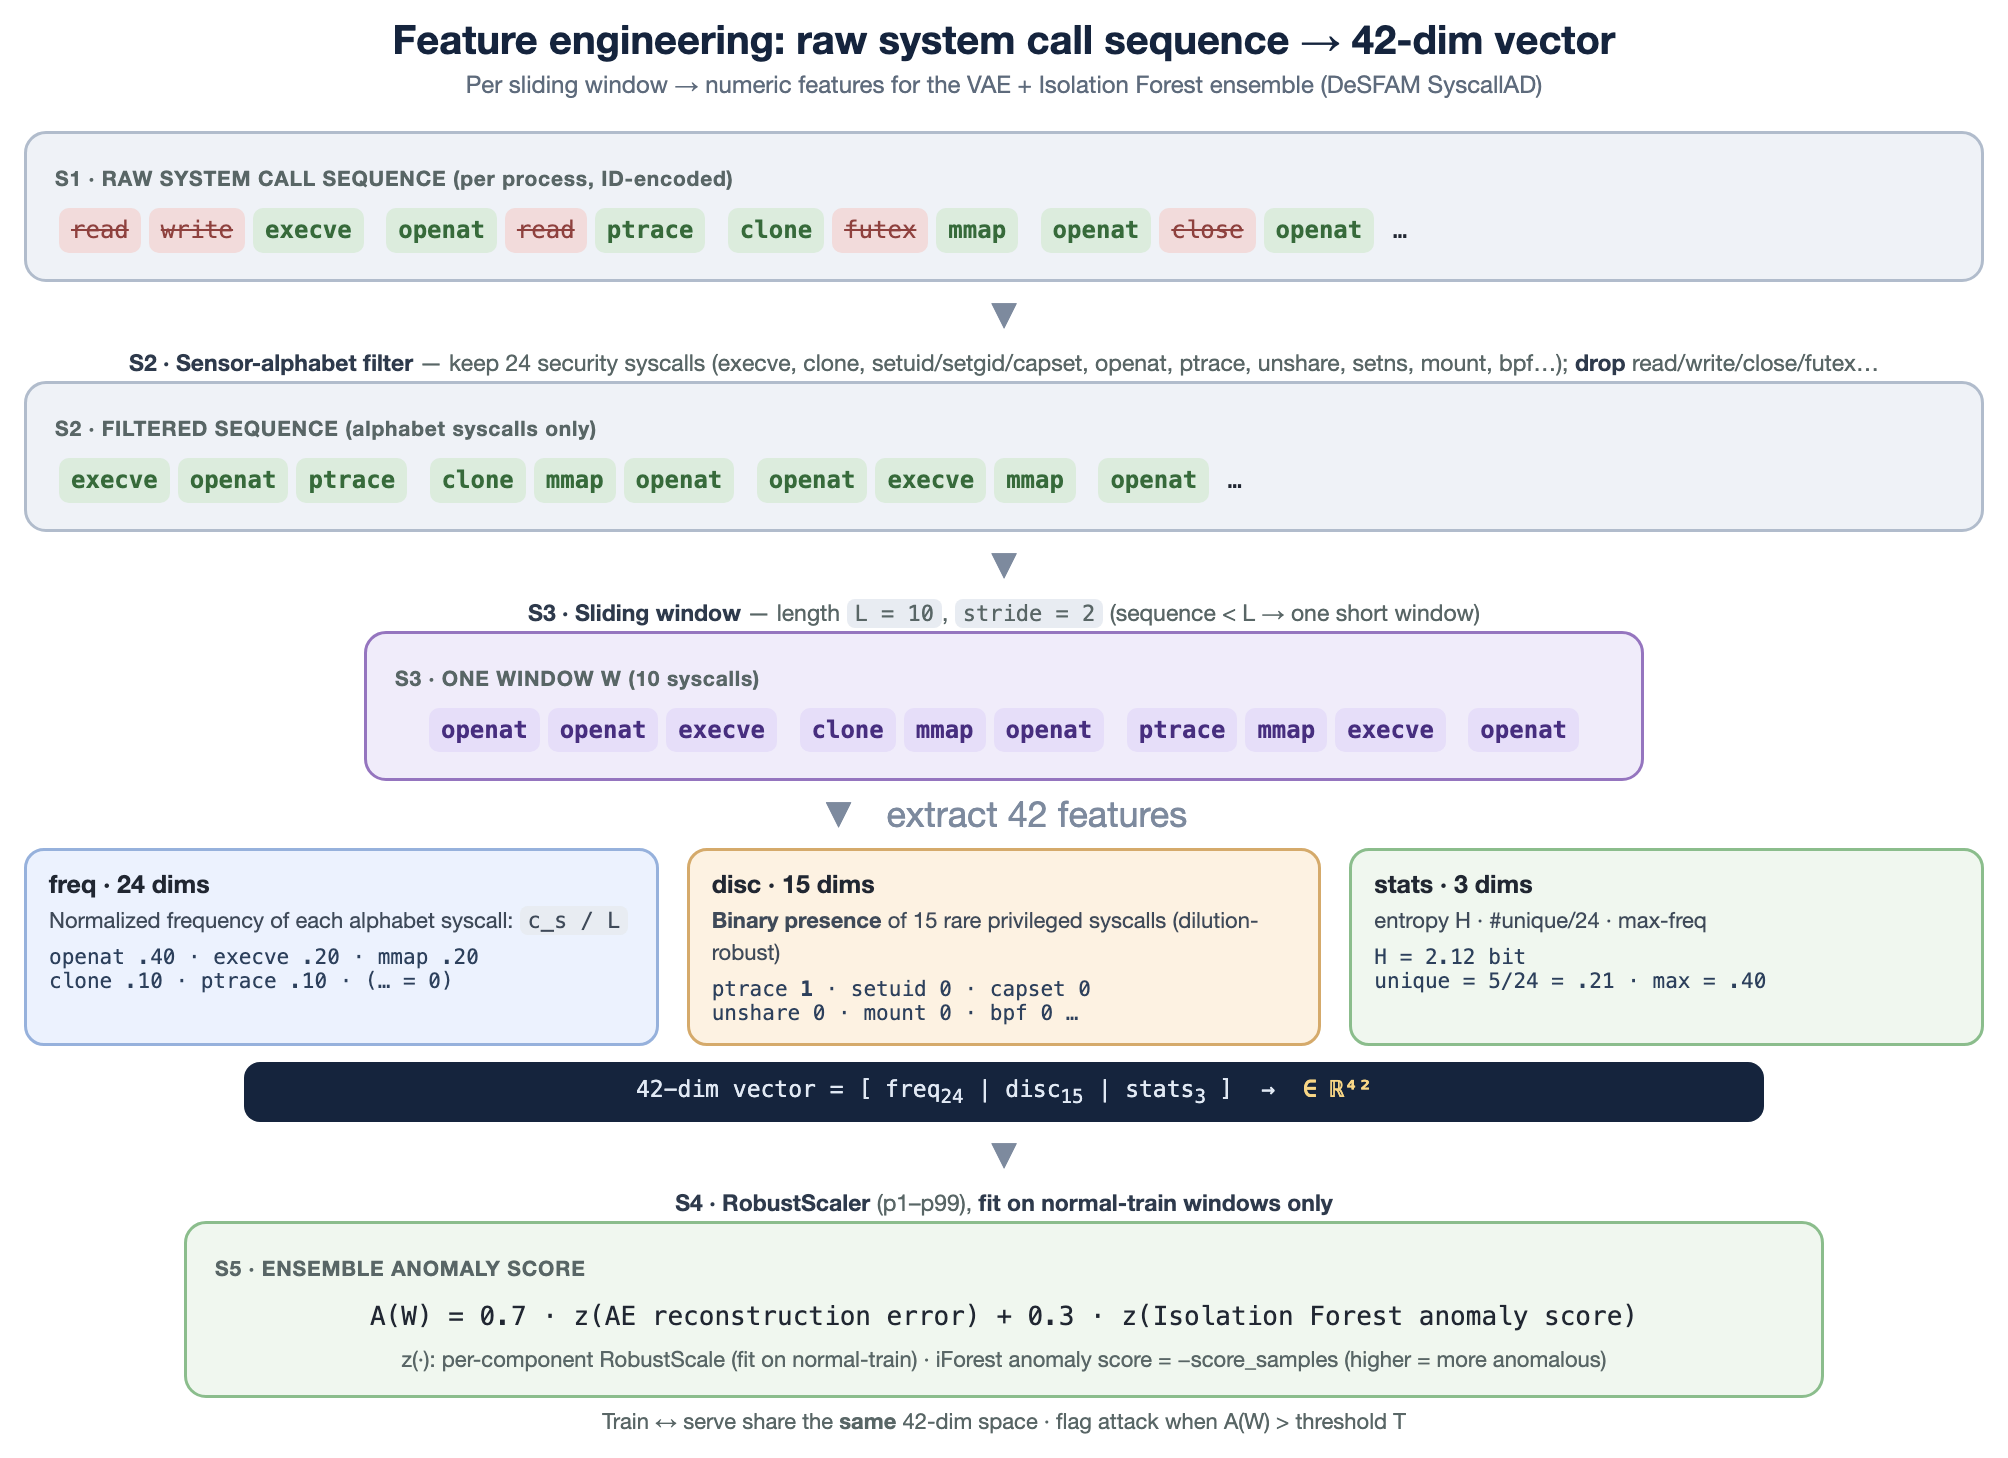
\includegraphics[width=0.96\textwidth]{figures/fig_features.png}
\caption{Quy trình trích xuất đặc trưng (ví dụ một cửa sổ).}
\label{fig:fe}
\end{figure}

\subsubsection{Bộ phát hiện (VAE + Isolation Forest)}
Bộ phát hiện được huấn luyện theo chế độ \textit{normal-only}, đúng theo thiết kế DeSFAM: một \textit{Variational Autoencoder} (VAE) và một Isolation Forest. VAE được cài bằng TensorFlow/Keras (encoder $42\to24\to$ latent $6$; huấn luyện Adam, 40 epoch); điểm bất thường của VAE là sai số tái tạo (reconstruction error) tính từ $z=\mu$. VAE ở đây được dựng lại theo \textit{kiến trúc} mô tả trong DeSFAM và huấn luyện lại trên DongTing; báo cáo không sử dụng mô hình đã huấn luyện sẵn (trọng số gốc) vì công trình gốc không phát hành chúng. Điểm của hai mô hình được RobustScale rồi hợp nhất theo trọng số $0{,}7/0{,}3$ thành anomaly score ensemble:
\[
A(W)=0{,}7\,z\big(\lVert g(\tilde{\mathbf{x}})-\tilde{\mathbf{x}}\rVert^2\big)+0{,}3\,z\big(-\mathrm{iForest}(\tilde{\mathbf{x}})\big),
\]
với $g$ là VAE (giải mã từ $z=\mu$) và $z(\cdot)$ là RobustScale từng thành phần (fit trên normal-train). Ngưỡng khởi tạo $T_0$ đặt tại phân vị $99{,}5$ của anomaly score lành tính (các mức ngưỡng $T_0/T_{op}/T_{\min}$ đã trình bày ở Mục~\ref{sec:method}).

\subsection{Mô hình mối đe doạ và hàng xóm gây nhiễu}
Kẻ tấn công được giả định đã có chỗ đứng trong một pod (post-exploitation) và thực hiện các kỹ thuật privilege escalation / container escape. Tấn công \textit{loud} (ồn) dùng nhiều system call đặc quyền dồn dập (anomaly score rất cao, $>$ phân vị $99{,}9$ lành tính); tấn công \textit{stealthy} (lén) rải mỏng (anomaly score chỉ vừa vượt operating point). \textit{Noisy neighbor} là một pod đồng trú sinh tải lành tính hỗn loạn (memory allocation, CPU, I/O), được mô hình hoá bằng các cửa sổ lành tính \textit{thực} của DongTing lấy theo dải phân vị anomaly score tăng dần: none ($\le$ phân vị 50), moderate (50--90), high ($>$ phân vị 90). Operating point $T_{op}$ đặt tại phân vị $95$ của anomaly score lành tính (FPR $\approx 5\%$); sàn EMA $T_{\min}$ đặt tại phân vị $50$.

\subsection{Quy trình ba phase và giao thức thí nghiệm}
\subsubsection{Ba phase tách biệt (đảm bảo độ tin cậy)}
Để loại bỏ rò rỉ (leakage) giữa calibration và đánh giá, pipeline được tách thành ba phase trên các tập dữ liệu \textit{rời rạc} (Hình~\ref{fig:pipeline}):
\begin{itemize}[leftmargin=1.2cm]
\item \textbf{Phase 1 — Training:} fit scaler, VAE, Isolation Forest và các component scaler \textit{chỉ} trên cửa sổ lành tính của tập train (50.877 cửa sổ), không nhiễm dữ liệu tấn công.
\item \textbf{Phase 2 — Calibration:} đặt các ngưỡng $T_0/T_{op}/T_{\min}$ cùng các mốc phân vị xác định dải noise và dải attack \textit{chỉ} trên tập calibration (½ benign-val + ½ attack).
\item \textbf{Phase 3 — Test:} chấm điểm, báo cáo AUC/AP và dựng các dòng thí nghiệm trên tập test \textit{rời rạc} với tập calibration (nửa còn lại).
\end{itemize}
Vì $\text{CAL}\cap\text{TEST}=\varnothing$, không có ngưỡng hay mốc phân vị nào được fit trên chính các cửa sổ dùng để đánh giá — qua đó loại bỏ calibration leakage và tăng độ tin cậy của kết luận.

\begin{figure}[ht]
\centering
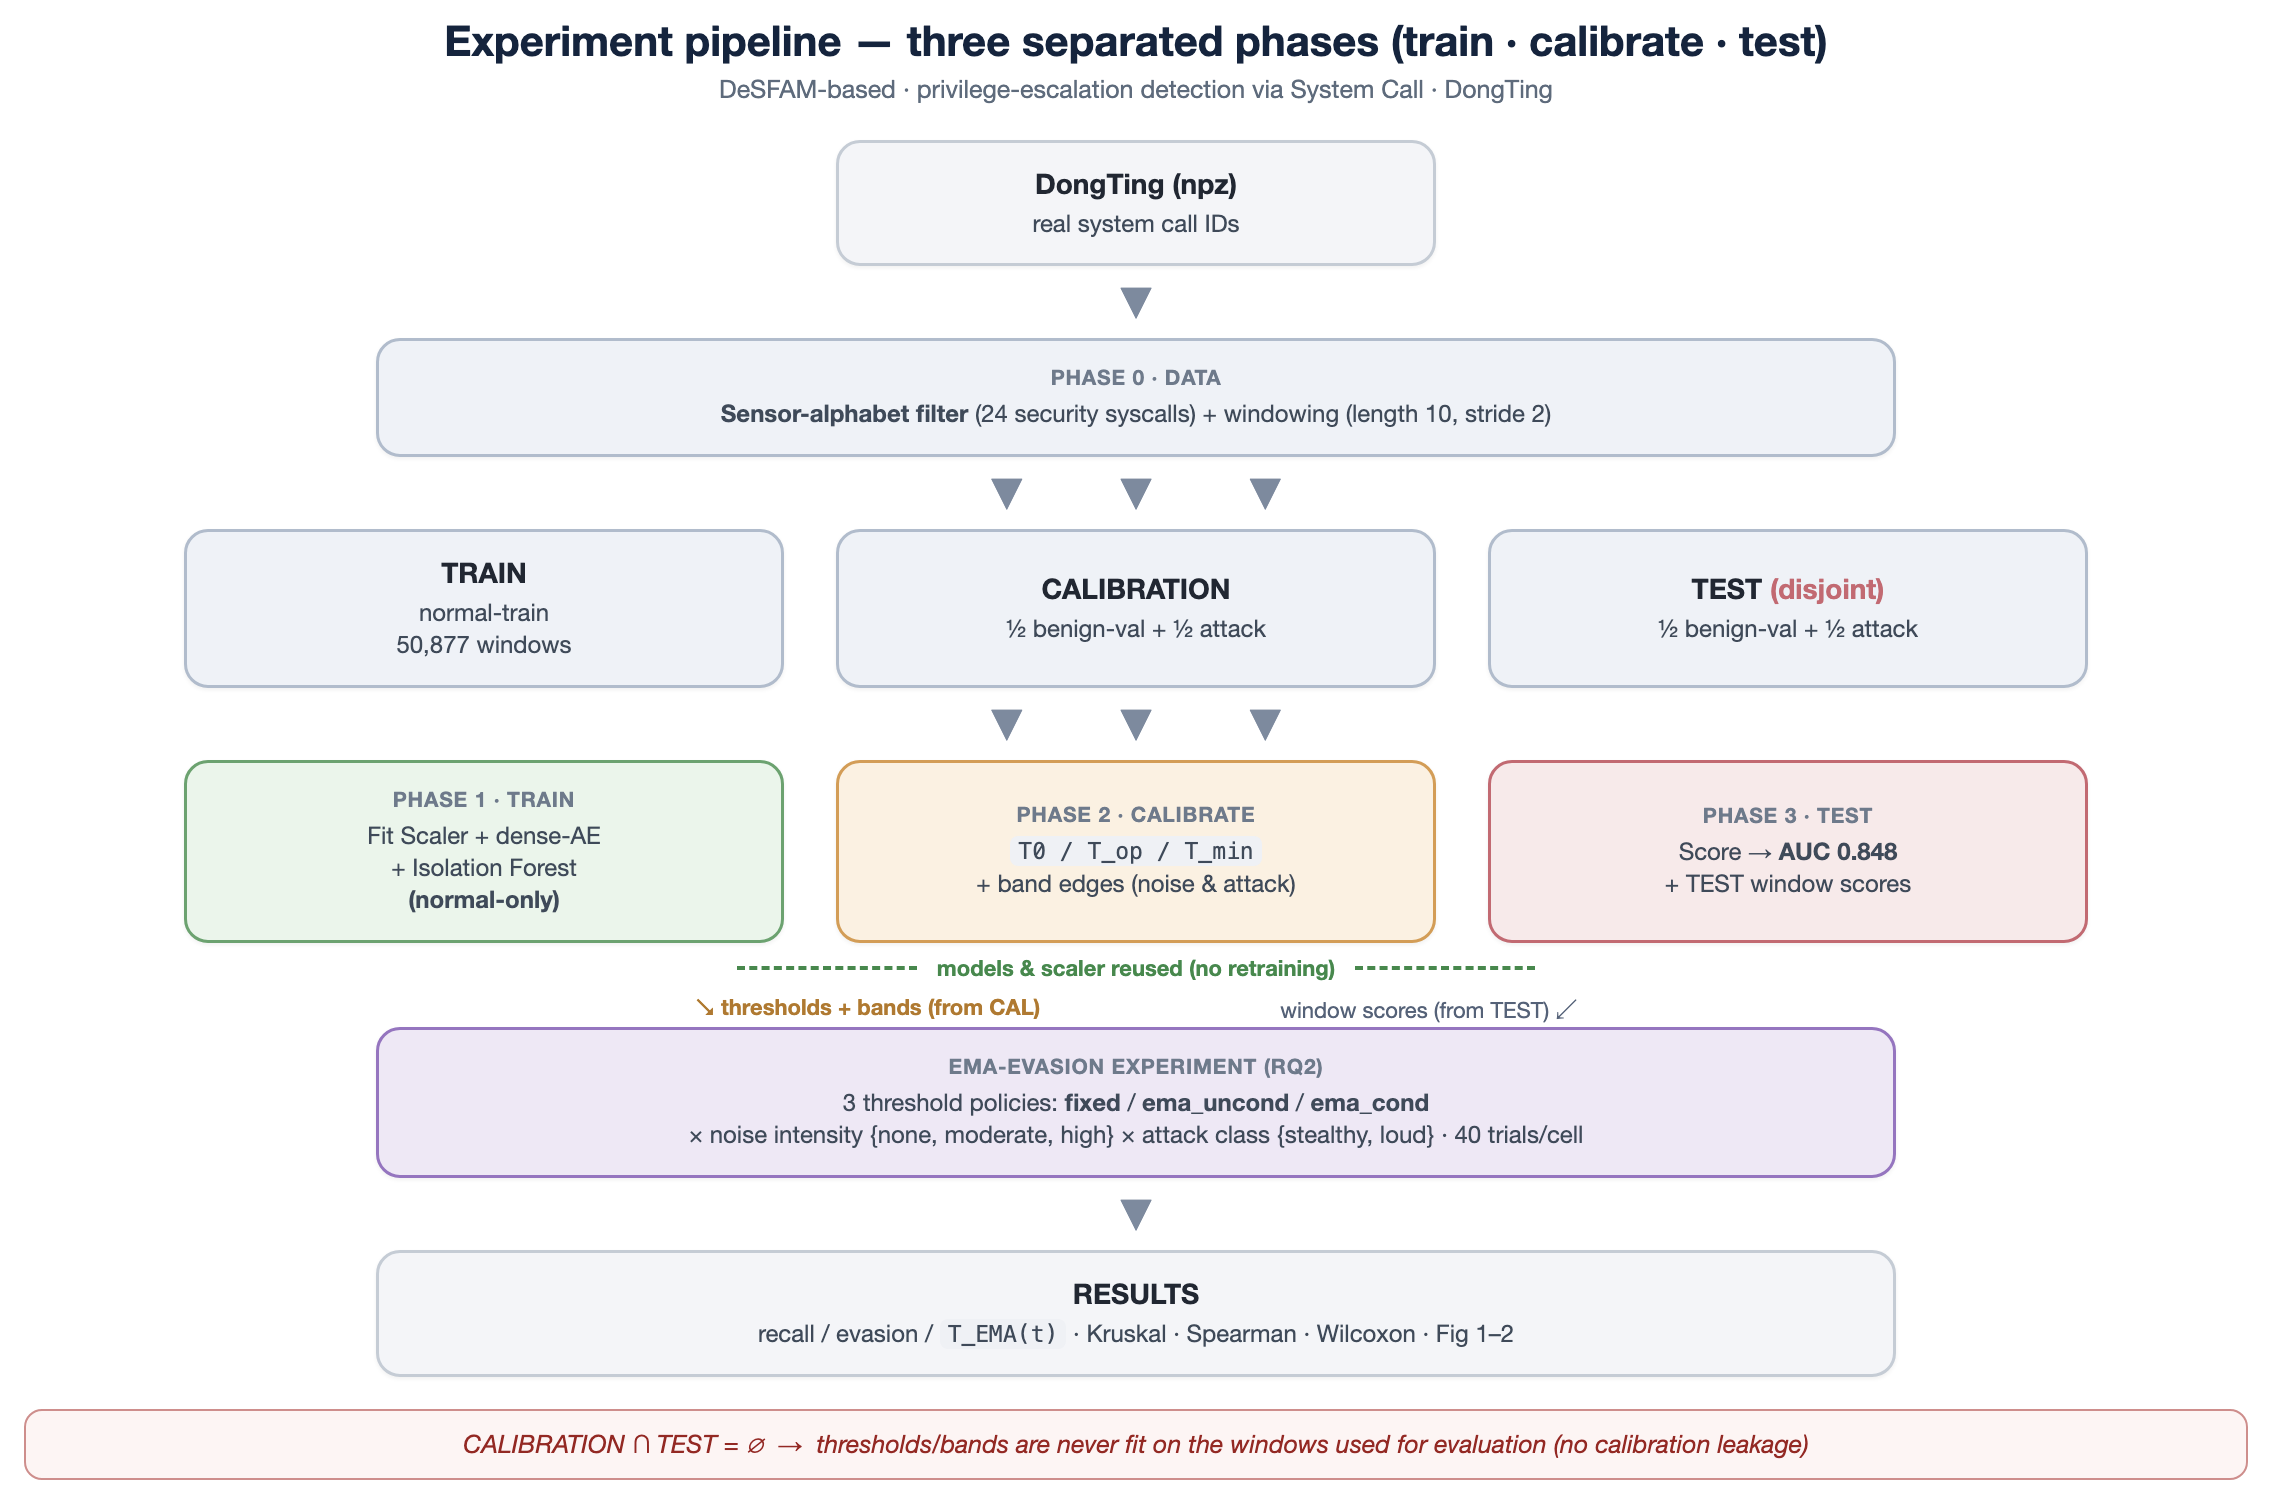
\includegraphics[width=0.92\textwidth]{figures/fig0_pipeline.png}
\caption{Pipeline thực nghiệm ba phase tách biệt ($\text{CAL}\cap\text{TEST}=\varnothing$).}
\label{fig:pipeline}
\end{figure}

\subsubsection{Cách tiến hành mỗi lượt thử (trial)}
Một \textit{trial} là một lượt chạy thí nghiệm độc lập trên một dòng cửa sổ tự dựng. Mỗi trial gồm các bước:
\begin{enumerate}[leftmargin=1.4cm]
\item \textbf{Dựng dòng cửa sổ TEST theo thứ tự thời gian:} warm-up (50 cửa sổ lành tính) $\to$ noise (150 cửa sổ, theo cường độ none/moderate/high) $\to$ attack (30 cửa sổ, theo loại stealthy/loud) — mô phỏng kịch bản vận hành bình thường, rồi hàng xóm bơm nhiễu, rồi tấn công xảy ra.
\item \textbf{Chạy cả ba chính sách ngưỡng} (\texttt{fixed}, \texttt{ema\_uncond}, \texttt{ema\_cond}) trên \textit{cùng} dòng cửa sổ đó để so sánh ghép cặp (cùng dữ liệu, chỉ khác chính sách).
\item \textbf{Lặp lại 40 trial} cho mỗi tổ hợp (loại tấn công $\times$ cường độ nhiễu).
\end{enumerate}
Cửa sổ trong mỗi trial được lấy mẫu \textit{có hoàn lại} từ các pool TEST hữu hạn (noise: $\approx$2530/1507/402 cửa sổ cho none/moderate/high; attack: $\approx$965 stealthy, $\approx$2883 loud); vì pool hữu hạn nên các trial không hoàn toàn độc lập — do đó CI bootstrap nên được đọc như chỉ báo, không phải sai số chuẩn chặt chẽ. Chi tiết tái lập ở Phụ lục~\ref{sec:repro}.
